\documentclass[10pt]{article}

\usepackage[letterpaper,margin=0.72in]{geometry}
\usepackage{amsmath,amssymb}
\usepackage{booktabs}
\usepackage{graphicx}
\usepackage{float}
\usepackage{hyperref}
\usepackage{longtable}
\usepackage{microtype}
\usepackage{multirow}
\usepackage{pdflscape}
\usepackage{xcolor}

\hypersetup{colorlinks=true,linkcolor=blue,citecolor=blue,urlcolor=blue}

\title{Supplementary Material\\
\large A Controlled Evaluation of Curvature-Inspired Scalar Feature Scaling
for Domain Generalization}
\author{Sunny Gupta \and Amit Sethi}
\date{}

\newcommand{\method}{\textsc{HyperDG}}
\newcommand{\pp}{\,pp}
\newcommand{\full}{\textsc{FullPerDomain}}
\newcommand{\erm}{\textsc{StandardERM}}
\newcommand{\shared}{\textsc{SharedLearnable}}
\newcommand{\novar}{\textsc{NoVariance}}

\begin{document}
\maketitle
\vspace{-1.8em}

\section{Scope and Evidence Status}
\label{sec:scope}

\paragraph{What the name refers to.}
\method{} denotes the exact scalar feature-scaling formulation evaluated in
the paper. It is not a citation to a separate external publication and it is
not a name for hyperbolic domain generalization in general. The paper and this
supplement specify the computation directly.

\paragraph{Claim boundary.}
The implementation performs scalar rescaling of Euclidean features during
training and unscaled Euclidean linear prediction. It is not a Lorentz or
Poincar\'e representation, a geodesic classifier, or a SAM inner loop. The
evidence below therefore addresses the executed scalar package and the need
for separate source-loader scalars. It does not address hyperbolic
representation learning in general.

\begin{table}[H]
\centering
\caption{Revision evidence inventory. Complete means every planned run reaches
the end of the declared training schedule and contributes to the reported
analysis.}
\label{tab:evidence-status}
\small
\begin{tabular}{p{0.27\linewidth}p{0.18\linewidth}p{0.47\linewidth}}
\toprule
Analysis & Status & Evidentiary use \\
\midrule
Six-condition controlled grid & Complete: 384/384 & Primary evidence:
six conditions, four datasets, four targets, and four run seeds. \\
Native DomainBed ERM & Complete: 64/64 & Whole-package utility comparator;
not a curvature-only causal contrast because the update routes differ. \\
Shared-learnable source scale & Complete: 64/64 & Direct domain-specificity
comparison with \novar{}; Frozen is not used as its substitute. \\
Source-only model selection & Complete & Primary endpoint; held-out target
accuracy is excluded from the frozen checkpoint score. \\
Target-clustered inference & Complete & Four targets are per-dataset clusters;
four datasets are suite clusters. \\
Post-hoc Poincar\'e projections & Excluded & Visualization only; not evidence
of manifold-valued training. \\
Legacy MERU attempts & Incomplete/excluded & Do not constitute a controlled
genuine-hyperbolic baseline and support no accuracy claim. \\
\bottomrule
\end{tabular}
\end{table}

\section{Frozen Revision Protocol}
\label{sec:protocol}

\subsection{Conditions}

All \method{}-path scale parameters ($a_i$ and the global $a_g$; see
Section~\ref{sec:audit}) start at zero, so every condition begins with
$c_i=c_g=\operatorname{softplus}(0)+10^{-4}=\log2+10^{-4}=0.6932472$, a feature
multiplier of $1/\sqrt{c}=1.2010358$. \textsc{MatchedControl} and
\textsc{Frozen} set the scale optimizer's learning rate to zero, so $a_i$ and
$a_g$ never move: $c_i=c_g=0.6932472$ is the fixed value applied at
\emph{every} update of the run, not only at initialization. \full{},
\novar{}, and \shared{} instead learn $a_i$ (or, for \shared{}, one shared
$a$) and $a_g$ from this same zero starting point with the separate scale
Adam optimizer described below. In a run with one held-out environment,
per-domain means one scalar for each of three source-loader slots, not four
persistent dataset-wide domain identities.

Only \erm{}, \full{}, \novar{}, and \shared{} enter the paper's two primary
suite contrasts (\full{}$-$\erm{} and \novar{}$-$\shared{}, both defined in
Section~\ref{sec:estimands-inference}). \textsc{MatchedControl} and \textsc{Frozen} are
secondary, descriptive diagnostics: no contrast reported in this paper treats
either condition as a primary inferential claim. \textsc{MatchedControl}
isolates what the \method{} update route costs or gains at fixed, non-learned
rescaling, before any auxiliary loss is active. \textsc{Frozen} is the
fixed-scale counterpart of \novar{}, letting learned and fixed scaling be
compared descriptively under the same non-dispersion auxiliary package; it is
not a substitute for \shared{}, since it changes learnability rather than
per-source specificity.

\begin{table}[H]
\centering
\caption{Exact identities of the six conditions. Coefficients are
$(\alpha_{\mathrm{var}},\beta_{\mathrm{align}},\gamma_{\mathrm{norm}},
\delta_{\mathrm{local}},\delta_{\mathrm{global}})$. Only the \erm{}, \full{},
\novar{}, and \shared{} rows enter the two primary contrasts;
\textsc{MatchedControl} and \textsc{Frozen} are descriptive.}
\label{tab:condition-identities}
\small
\setlength{\tabcolsep}{4pt}
\begin{tabular}{p{0.18\linewidth}p{0.21\linewidth}p{0.16\linewidth}p{0.32\linewidth}}
\toprule
Condition & Scales & Coefficients & Interpretation \\
\midrule
\erm{} & None & n/a & Native concatenated-minibatch DomainBed ERM. \\
\textsc{MatchedControl} & Three local plus global, all fixed at $0.6932472$ &
$(0,0,0,0,0)$ & \method{} route with auxiliary losses disabled; fixed feature
rescaling remains. Descriptive only. \\
\full{} & Three local plus global, learned &
$(.2,.5,.05,.1,.1)$ & Complete submitted implementation. \\
\textsc{Frozen} & Three local plus global, fixed at $0.6932472$ &
$(0,.5,.05,.1,.1)$ & Non-dispersion auxiliary package with fixed scales.
Descriptive only. \\
\novar{} & Three local plus global, learned &
$(0,.5,.05,.1,.1)$ & Removes only explicit between-scale dispersion from
\full{}. \\
\shared{} & One shared local plus separate global, learned &
$(.2,.5,.05,.1,.1)$ & Dispersion is structurally zero despite $\alpha=.2$;
clean comparator for \novar{}. \\
\bottomrule
\end{tabular}
\end{table}

\subsection{Data, targets, and training}

\begin{table}[H]
\centering
\caption{Named held-out targets. Every target is evaluated with seeds 0--3.}
\label{tab:target-map}
\small
\begin{tabular}{lllll}
\toprule
Dataset & Target 0 & Target 1 & Target 2 & Target 3 \\
\midrule
PACS & ArtPainting & Cartoon & Photo & Sketch \\
VLCS & Caltech101 & LabelMe & SUN09 & VOC2007 \\
OfficeHome & Art & Clipart & Product & RealWorld \\
TerraIncognita & L100 & L38 & L43 & L46 \\
\bottomrule
\end{tabular}
\end{table}

All conditions use the same environment partitions and
deterministic seed-dependent 80/20 splits, data augmentation,
\texttt{timm} \texttt{resnet50.ram\_in1k} ImageNet weights, 2,048-dimensional
features, a biased linear classifier, batch size 32 per source, 5,000 updates,
Adam network learning rate $5\times10^{-5}$, zero weight decay, and evaluation
every 200 updates plus update 4999. Seeds change the split, initialization,
minibatch order, and augmentation randomness. BatchNorm is active and dropout
is zero. Learned scale parameters use Adam at $10^{-4}$; the \method{} route
clips network and scale gradient norms to 5.

\emph{Native DomainBed ERM} means the unmodified upstream DomainBed
\texttt{ERM} class, run inside this project's identical data, split,
augmentation, timm-ResNet-50, and source-only-selection harness: it
concatenates the three source minibatches into one 96-example batch, computes
one cross-entropy loss, and takes one Adam step with one optimizer and no
gradient clipping. ``Native'' describes the update rule and objective, not a
claim that the surrounding training/evaluation code is an untouched upstream
DomainBed installation.

Per training step, the \method{} route calls the feature extractor six times:
three source-minibatch forward passes (with gradients) build the training
objective in Equation~(2) of the main paper, and, after the optimizer step,
three further forward passes under \texttt{torch.no\_grad()} recompute
training accuracy for logging. \texttt{no\_grad()} disables gradient
tracking only; it does \emph{not} switch the model to \texttt{eval()}, and
the training loop never calls \texttt{eval()} during an update. All six
forward passes therefore run with the model in ordinary training mode, and
BatchNorm's running mean, running variance, and batch counter update exactly
as they would for any other training-mode forward pass -- including the three
no-gradient diagnostic passes. Native ERM instead calls the feature extractor
once per step, on the concatenated 96-example batch, so it updates BatchNorm
statistics from one training-mode forward pass rather than \method{}'s six.
This asymmetry, together with the separate scale optimizer and gradient
clipping described above, is why \full{}$-$\erm{} is a complete-package
comparison rather than an isolated curvature effect. Both sides of
\novar{}$-$\shared{} use the identical \method{} route, so this asymmetry
cancels out of that contrast.

\subsection{Target-excluding checkpoint selection}

For method $m$, dataset $j$, held-out target $d$, run seed $s$, source
environment $r$, and checkpoint $t$, let $V_{mjdsrt}$ be source
\texttt{out}-split accuracy. The selected checkpoint is
\begin{equation}
t^*_{mjds}=\arg\max_t\frac{1}{3}\sum_{r\ne d}V_{mjdsrt},
\end{equation}
with earliest-checkpoint tie breaking. The held-out target key is not used in
this calculation; its accuracy is read only after $t^*$ is fixed. The trainer
logged target values at every checkpoint, so we do not make the stronger claim
that target curves never existed. Source validation inherits stochastic
augmentation and is evaluated once per logged checkpoint.

\subsection{Estimand}
\label{sec:estimand}

Every suite-level number in this supplement and the main paper is a claim
about the equal-weighted macro over exactly PACS, VLCS, OfficeHome, and
TerraIncognita under this protocol. It is not a claim about a population or
superpopulation of DG tasks that these four benchmarks are sampled from: the
suite was chosen for heterogeneous shift type (style, acquisition, context,
and camera location; Section~\ref{sec:protocol}), not as a random draw from a
larger task distribution. Figure~1 of the main paper states this explicitly
because the suite-level interval, sign-flip test, and TOST below use the four
dataset effects as inferential clusters without implying that conclusions
transfer to DG tasks outside this fixed suite.

\subsection{Estimands and inference}
\label{sec:estimands-inference}

For a treatment $A$ and comparator $B$, define
\begin{equation}
g_{jds}=Y_{Ajds}-Y_{Bjds},\qquad
\bar g_{jd}=\frac14\sum_sg_{jds},\qquad
\Delta_j=\frac14\sum_d\bar g_{jd}.
\end{equation}
Seeds are averaged within target first ($\bar g_{jd}$), and targets are
averaged within dataset second ($\Delta_j$). The suite-level procedures below
consume only the resulting four dataset means $\Delta_j$; they do not
separately repropagate within-target seed variance or between-target
variance into the suite-level interval or test. Those lower-level components
are real and are reported descriptively -- per-target effects in
Table~\ref{tab:target-effects}, and the target/seed/residual decomposition in
Table~\ref{tab:effect-variability} -- but they contribute to the suite-level
uncertainty only through the four dataset means they produce, not as an
additional variance term added at the suite level.

Inference within dataset $j$ uses the four $\bar g_{jd}$ values, not the 16
seed-by-target cells. We enumerate all $2^4=16$ target-level sign
assignments for an exact two-sided sign-flip test and separately report a
$t_3$ interval. The sign-flip test is exact conditional on treating the four
target-level signs as exchangeable under the joint no-effect null, i.e.\ that
all 16 sign patterns are equally likely if each $\bar g_{jd}$ is symmetric
about zero under the null. This is a working symmetry assumption suited to a
four-cluster benchmark suite; it does not assume the datasets were randomly
sampled or randomly assigned, and it is not a test of whether dataset-level
effects cancel under a suite-macro-only null. The minimum attainable
two-sided exact $p$-value is therefore .125 with four clusters. The suite
macro averages the four $\Delta_j$ values and uses the four datasets as
clusters. The two primary suite contrasts form a Holm-2 family; eight
per-dataset contrasts are a separate sensitivity family.

We declare the exact sign-flip test with Holm correction as the primary
inferential procedure for both suite-level difference claims. The $t_3$
interval and the four-cluster bootstrap sensitivity are secondary: they are
working-model summaries that lean on approximate normality or resampling
validity with only four clusters, and they do not override the primary
result when the two disagree, as they do for \full{}$-$\erm{}
(Table~\ref{tab:primary-suite}: $t_3$ 95\% CI excludes zero, exact $p=.125$,
Holm $p=.250$).

The revision-stage SESOI is $\pm1\pp$, selected after the originally submitted
results were known but before the 128 added ERM/shared runs completed.
Equivalence requires the clustered 90\% interval to lie wholly inside that
margin. Margins of $\pm0.5$ and $\pm2\pp$ are sensitivities. TOST, like the
$t_3$ interval, is a secondary working-model summary conditional on the same
fixed four-dataset macro (Section~\ref{sec:estimand}); failure to pass TOST is
inconclusive, not evidence of nonequivalence, and a pass supports equivalence
only for that fixed-suite macro.

\section{Complete Source-Selected Results}
\label{sec:complete-results}

\subsection{Six-condition summary with separated variability}

Table~\ref{tab:six-condition} separates between-target SD from the root-mean
square within-target run-seed SD. The latter combines split, initialization,
minibatch-order, and augmentation randomness; it is not a pure optimization
seed SD.

\begin{table}[H]
\centering
\caption{Source-selected accuracy and two distinct variability components.
Accuracy is the equal-target macro mean.}
\label{tab:six-condition}
\resizebox{\textwidth}{!}{%
% Generated by HyperDG2/scripts/render_review_results.py.
% Requires \usepackage{booktabs}.
\begin{tabular}{llrrr}
\toprule
Condition & Dataset & Accuracy (\%) & Between-target SD & Within-target run-seed SD (RMS) \\
\midrule
Standard ERM & PACS & 85.88 & 7.98 & 3.04 \\
Standard ERM & VLCS & 77.19 & 14.09 & 1.49 \\
Standard ERM & OfficeHome & 70.21 & 10.90 & 1.79 \\
Standard ERM & TerraIncognita & 47.13 & 6.62 & 4.33 \\
Matched control & PACS & 84.22 & 7.99 & 3.39 \\
Matched control & VLCS & 75.38 & 15.07 & 2.44 \\
Matched control & OfficeHome & 70.05 & 10.73 & 2.31 \\
Matched control & TerraIncognita & 44.14 & 8.70 & 4.21 \\
Full per-domain & PACS & 84.87 & 8.19 & 1.89 \\
Full per-domain & VLCS & 76.42 & 14.90 & 1.65 \\
Full per-domain & OfficeHome & 68.52 & 10.33 & 2.54 \\
Full per-domain & TerraIncognita & 44.17 & 4.60 & 4.28 \\
Frozen & PACS & 86.14 & 7.22 & 2.19 \\
Frozen & VLCS & 75.84 & 14.30 & 2.22 \\
Frozen & OfficeHome & 67.81 & 11.91 & 1.57 \\
Frozen & TerraIncognita & 44.20 & 6.98 & 3.41 \\
No-variance per-domain & PACS & 85.28 & 7.76 & 2.00 \\
No-variance per-domain & VLCS & 76.17 & 14.95 & 1.19 \\
No-variance per-domain & OfficeHome & 68.36 & 10.10 & 2.64 \\
No-variance per-domain & TerraIncognita & 43.70 & 7.90 & 4.72 \\
Shared learnable & PACS & 85.55 & 7.54 & 3.01 \\
Shared learnable & VLCS & 76.56 & 14.65 & 2.20 \\
Shared learnable & OfficeHome & 68.17 & 11.15 & 2.09 \\
Shared learnable & TerraIncognita & 43.75 & 5.35 & 4.73 \\
\bottomrule
\end{tabular}
}
\end{table}

Across the 24 condition-by-dataset cells, between-target SD ranges from
$4.60$ to $15.07\pp$, while within-target run-seed SD (RMS) ranges from
$1.19$ to $4.73\pp$. Pooling these sources into one SD would obscure the
dominant target-difficulty variation in several datasets.

\subsection{Every target and all four run seeds}

\begin{landscape}
\setlength{\tabcolsep}{4pt}
\scriptsize
% Generated by HyperDG2/scripts/render_review_results.py.
% Requires \usepackage{booktabs,longtable}.
\begin{longtable}{lllrrrrrr}
\caption{Every source-selected held-out-target accuracy, with all four run
seeds, target mean, and run-seed SD.}
\label{tab:all-target-accuracies}\\
\toprule
Condition & Dataset & Target & Seed 0 & Seed 1 & Seed 2 & Seed 3 & Mean & Run-seed SD \\
\midrule
\endfirsthead
\toprule
Condition & Dataset & Target & Seed 0 & Seed 1 & Seed 2 & Seed 3 & Mean & Run-seed SD \\
\midrule
\endhead
\bottomrule
\endlastfoot
Standard ERM & PACS & ArtPainting & 83.62 & 91.93 & 81.17 & 86.80 & 85.88 & 4.64 \\
Standard ERM & PACS & Cartoon & 82.69 & 81.62 & 79.70 & 75.43 & 79.86 & 3.20 \\
Standard ERM & PACS & Photo & 99.40 & 97.01 & 97.01 & 95.21 & 97.16 & 1.72 \\
Standard ERM & PACS & Sketch & 82.17 & 78.73 & 81.27 & 80.38 & 80.64 & 1.47 \\
Standard ERM & VLCS & Caltech101 & 98.59 & 96.11 & 95.76 & 97.17 & 96.91 & 1.27 \\
Standard ERM & VLCS & LabelMe & 66.42 & 63.21 & 64.53 & 62.83 & 64.25 & 1.62 \\
Standard ERM & VLCS & SUN09 & 71.19 & 69.36 & 71.34 & 71.80 & 70.92 & 1.07 \\
Standard ERM & VLCS & VOC2007 & 78.52 & 75.70 & 77.93 & 74.52 & 76.67 & 1.88 \\
Standard ERM & OfficeHome & Art & 67.01 & 64.54 & 64.54 & 66.39 & 65.62 & 1.28 \\
Standard ERM & OfficeHome & Clipart & 57.16 & 53.15 & 58.53 & 59.11 & 56.99 & 2.69 \\
Standard ERM & OfficeHome & Product & 79.93 & 78.58 & 77.00 & 77.11 & 78.16 & 1.38 \\
Standard ERM & OfficeHome & RealWorld & 80.25 & 78.19 & 80.25 & 81.63 & 80.08 & 1.42 \\
Standard ERM & TerraIncognita & L100 & 45.85 & 47.38 & 46.15 & 57.33 & 49.18 & 5.48 \\
Standard ERM & TerraIncognita & L38 & 48.08 & 49.31 & 42.45 & 36.05 & 43.97 & 6.07 \\
Standard ERM & TerraIncognita & L43 & 56.09 & 54.98 & 53.11 & 57.09 & 55.32 & 1.71 \\
Standard ERM & TerraIncognita & L46 & 42.32 & 40.20 & 36.93 & 40.77 & 40.05 & 2.27 \\
Matched control & PACS & ArtPainting & 86.06 & 86.55 & 82.15 & 83.86 & 84.66 & 2.04 \\
Matched control & PACS & Cartoon & 81.84 & 79.70 & 77.14 & 73.93 & 78.15 & 3.41 \\
Matched control & PACS & Photo & 96.11 & 93.71 & 95.81 & 95.81 & 95.36 & 1.11 \\
Matched control & PACS & Sketch & 83.18 & 82.93 & 71.97 & 76.69 & 78.69 & 5.39 \\
Matched control & VLCS & Caltech101 & 95.41 & 96.11 & 96.11 & 98.23 & 96.47 & 1.22 \\
Matched control & VLCS & LabelMe & 60.75 & 61.13 & 59.62 & 61.32 & 60.71 & 0.76 \\
Matched control & VLCS & SUN09 & 74.09 & 70.58 & 72.87 & 72.87 & 72.60 & 1.46 \\
Matched control & VLCS & VOC2007 & 74.96 & 75.41 & 70.67 & 65.93 & 71.74 & 4.43 \\
Matched control & OfficeHome & Art & 64.12 & 65.15 & 62.27 & 69.69 & 65.31 & 3.16 \\
Matched control & OfficeHome & Clipart & 59.11 & 53.61 & 56.47 & 59.34 & 57.13 & 2.68 \\
Matched control & OfficeHome & Product & 78.80 & 80.27 & 78.92 & 76.44 & 78.61 & 1.59 \\
Matched control & OfficeHome & RealWorld & 78.65 & 77.61 & 80.02 & 80.37 & 79.16 & 1.27 \\
Matched control & TerraIncognita & L100 & 58.46 & 49.23 & 56.51 & 57.64 & 55.46 & 4.23 \\
Matched control & TerraIncognita & L38 & 42.55 & 47.31 & 42.45 & 33.44 & 41.44 & 5.80 \\
Matched control & TerraIncognita & L43 & 42.66 & 50.37 & 43.53 & 43.66 & 45.06 & 3.57 \\
Matched control & TerraIncognita & L46 & 38.07 & 35.13 & 32.19 & 33.09 & 34.62 & 2.61 \\
Full per-domain & PACS & ArtPainting & 84.11 & 85.33 & 83.62 & 83.86 & 84.23 & 0.76 \\
Full per-domain & PACS & Cartoon & 78.85 & 78.85 & 76.28 & 76.71 & 77.67 & 1.37 \\
Full per-domain & PACS & Photo & 95.51 & 97.31 & 96.71 & 96.41 & 96.48 & 0.75 \\
Full per-domain & PACS & Sketch & 81.40 & 85.61 & 79.75 & 77.71 & 81.11 & 3.35 \\
Full per-domain & VLCS & Caltech101 & 99.29 & 96.47 & 97.17 & 96.82 & 97.44 & 1.27 \\
Full per-domain & VLCS & LabelMe & 62.08 & 62.26 & 62.83 & 62.08 & 62.31 & 0.36 \\
Full per-domain & VLCS & SUN09 & 73.32 & 69.82 & 73.93 & 71.65 & 72.18 & 1.85 \\
Full per-domain & VLCS & VOC2007 & 75.70 & 75.41 & 73.33 & 70.52 & 73.74 & 2.39 \\
Full per-domain & OfficeHome & Art & 65.36 & 62.27 & 56.91 & 65.36 & 62.47 & 3.99 \\
Full per-domain & OfficeHome & Clipart & 55.90 & 55.21 & 57.96 & 59.22 & 57.07 & 1.85 \\
Full per-domain & OfficeHome & Product & 79.26 & 79.14 & 74.75 & 76.21 & 77.34 & 2.23 \\
Full per-domain & OfficeHome & RealWorld & 76.46 & 76.00 & 78.87 & 77.38 & 77.18 & 1.27 \\
Full per-domain & TerraIncognita & L100 & 48.00 & 44.82 & 55.28 & 48.31 & 49.10 & 4.41 \\
Full per-domain & TerraIncognita & L38 & 34.10 & 44.91 & 43.16 & 39.27 & 40.36 & 4.79 \\
Full per-domain & TerraIncognita & L43 & 40.42 & 49.50 & 48.88 & 49.50 & 47.08 & 4.45 \\
Full per-domain & TerraIncognita & L46 & 42.65 & 35.62 & 39.62 & 42.65 & 40.13 & 3.33 \\
Frozen & PACS & ArtPainting & 88.26 & 88.51 & 84.11 & 83.86 & 86.19 & 2.54 \\
Frozen & PACS & Cartoon & 84.19 & 77.78 & 77.35 & 79.06 & 79.59 & 3.15 \\
Frozen & PACS & Photo & 95.81 & 95.51 & 96.71 & 96.71 & 96.18 & 0.62 \\
Frozen & PACS & Sketch & 82.17 & 84.59 & 82.68 & 80.89 & 82.58 & 1.53 \\
Frozen & VLCS & Caltech101 & 98.23 & 94.70 & 96.82 & 95.05 & 96.20 & 1.64 \\
Frozen & VLCS & LabelMe & 62.83 & 65.66 & 61.13 & 61.32 & 62.74 & 2.09 \\
Frozen & VLCS & SUN09 & 74.54 & 68.45 & 74.70 & 73.32 & 72.75 & 2.94 \\
Frozen & VLCS & VOC2007 & 70.37 & 74.22 & 72.30 & 69.78 & 71.67 & 2.01 \\
Frozen & OfficeHome & Art & 62.06 & 61.03 & 60.82 & 63.30 & 61.80 & 1.13 \\
Frozen & OfficeHome & Clipart & 53.95 & 52.00 & 55.33 & 54.64 & 53.98 & 1.43 \\
Frozen & OfficeHome & Product & 78.92 & 75.99 & 77.00 & 76.44 & 77.09 & 1.29 \\
Frozen & OfficeHome & RealWorld & 76.23 & 76.81 & 79.79 & 80.71 & 78.39 & 2.20 \\
Frozen & TerraIncognita & L100 & 55.18 & 46.67 & 49.33 & 57.23 & 52.10 & 4.93 \\
Frozen & TerraIncognita & L38 & 37.79 & 42.75 & 40.91 & 37.79 & 39.81 & 2.45 \\
Frozen & TerraIncognita & L43 & 43.66 & 45.77 & 50.00 & 51.99 & 47.85 & 3.82 \\
Frozen & TerraIncognita & L46 & 36.36 & 36.52 & 36.44 & 38.89 & 37.05 & 1.23 \\
No-variance per-domain & PACS & ArtPainting & 83.62 & 82.89 & 87.53 & 82.89 & 84.23 & 2.23 \\
No-variance per-domain & PACS & Cartoon & 79.27 & 77.56 & 77.56 & 77.99 & 78.10 & 0.81 \\
No-variance per-domain & PACS & Photo & 97.60 & 94.61 & 95.81 & 97.01 & 96.26 & 1.33 \\
No-variance per-domain & PACS & Sketch & 84.71 & 85.22 & 79.11 & 81.15 & 82.55 & 2.92 \\
No-variance per-domain & VLCS & Caltech101 & 97.88 & 97.17 & 96.82 & 98.23 & 97.53 & 0.65 \\
No-variance per-domain & VLCS & LabelMe & 63.02 & 63.21 & 63.96 & 60.38 & 62.64 & 1.56 \\
No-variance per-domain & VLCS & SUN09 & 72.26 & 71.04 & 72.56 & 70.73 & 71.65 & 0.90 \\
No-variance per-domain & VLCS & VOC2007 & 73.63 & 73.93 & 73.04 & 70.81 & 72.85 & 1.41 \\
No-variance per-domain & OfficeHome & Art & 60.62 & 59.38 & 68.25 & 60.41 & 62.16 & 4.09 \\
No-variance per-domain & OfficeHome & Clipart & 57.27 & 54.07 & 56.82 & 61.40 & 57.39 & 3.02 \\
No-variance per-domain & OfficeHome & Product & 76.89 & 78.69 & 75.99 & 75.99 & 76.89 & 1.28 \\
No-variance per-domain & OfficeHome & RealWorld & 77.04 & 76.35 & 76.92 & 77.61 & 76.98 & 0.52 \\
No-variance per-domain & TerraIncognita & L100 & 60.10 & 52.41 & 51.59 & 46.77 & 52.72 & 5.52 \\
No-variance per-domain & TerraIncognita & L38 & 39.22 & 35.28 & 44.55 & 33.08 & 38.03 & 5.03 \\
No-variance per-domain & TerraIncognita & L43 & 49.25 & 43.66 & 47.39 & 51.12 & 47.85 & 3.19 \\
No-variance per-domain & TerraIncognita & L46 & 43.06 & 32.68 & 35.95 & 33.09 & 36.19 & 4.80 \\
Shared learnable & PACS & ArtPainting & 80.68 & 88.26 & 84.84 & 87.04 & 85.21 & 3.33 \\
Shared learnable & PACS & Cartoon & 83.33 & 79.91 & 75.00 & 77.35 & 78.90 & 3.57 \\
Shared learnable & PACS & Photo & 97.31 & 97.31 & 95.81 & 94.31 & 96.18 & 1.43 \\
Shared learnable & PACS & Sketch & 84.08 & 84.84 & 77.83 & 80.89 & 81.91 & 3.21 \\
Shared learnable & VLCS & Caltech101 & 97.88 & 97.17 & 96.11 & 97.88 & 97.26 & 0.83 \\
Shared learnable & VLCS & LabelMe & 65.85 & 59.81 & 64.15 & 61.51 & 62.83 & 2.69 \\
Shared learnable & VLCS & SUN09 & 73.02 & 68.75 & 74.39 & 71.65 & 71.95 & 2.41 \\
Shared learnable & VLCS & VOC2007 & 76.59 & 75.85 & 72.30 & 72.00 & 74.19 & 2.37 \\
Shared learnable & OfficeHome & Art & 61.03 & 59.18 & 63.09 & 64.95 & 62.06 & 2.50 \\
Shared learnable & OfficeHome & Clipart & 57.04 & 52.46 & 53.84 & 58.76 & 55.53 & 2.89 \\
Shared learnable & OfficeHome & Product & 78.58 & 79.26 & 76.10 & 76.78 & 77.68 & 1.48 \\
Shared learnable & OfficeHome & RealWorld & 76.46 & 78.19 & 77.15 & 77.84 & 77.41 & 0.76 \\
Shared learnable & TerraIncognita & L100 & 57.54 & 46.77 & 49.23 & 45.03 & 49.64 & 5.54 \\
Shared learnable & TerraIncognita & L38 & 44.75 & 47.52 & 38.76 & 33.69 & 41.18 & 6.19 \\
Shared learnable & TerraIncognita & L43 & 45.15 & 41.79 & 50.50 & 48.63 & 46.52 & 3.85 \\
Shared learnable & TerraIncognita & L46 & 40.77 & 34.97 & 37.99 & 36.93 & 37.66 & 2.42 \\
\end{longtable}

\end{landscape}

\noindent
The preceding table is the complete 384-cell accuracy inventory: six
conditions, four datasets, four named targets, and four seeds. Values are the
held-out target \texttt{out}-split accuracies at the source-selected
checkpoint. No target or seed is omitted.

\section{Primary Contrasts and Small-Cluster Inference}
\label{sec:inference}

\subsection{Suite and per-dataset estimates}

\begin{table}[H]
\centering
\caption{Primary suite-macro analyses. Exact tests flip the four dataset
effects; Holm adjusts the two exact $p$-values. TOST uses the revision-stage
$\pm1\pp$ margin.}
\label{tab:primary-suite}
\small
\setlength{\tabcolsep}{4pt}
\begin{tabular}{lrrrrrr}
\toprule
Contrast & Effect & 95\% CI & Exact $p$ & Holm $p$ & 90\% CI & TOST $p$ \\
\midrule
\full{}$-$\erm{} & $-1.61$ & $[-3.17,-0.04]$ & .125 & .250 &
$[-2.77,-0.45]$ & .848 \\
\novar{}$-$\shared{} & $-0.13$ & $[-0.53,0.27]$ & .375 & .375 &
$[-0.43,0.17]$ & .003 \\
\bottomrule
\end{tabular}
\end{table}

\begin{table}[H]
\centering
\caption{Per-dataset target-clustered sensitivities. Holm adjusts these eight
exact tests as a sensitivity family. No row establishes equivalence within
$\pm1\pp$.}
\label{tab:primary-datasets}
\scriptsize
\setlength{\tabcolsep}{3.5pt}
\begin{tabular}{llrrrrrr}
\toprule
Contrast & Dataset & Effect & 95\% CI & Exact $p$ & Holm $p$ & 90\% CI & TOST $p$ \\
\midrule
\full{}$-$\erm{} & PACS & $-1.01$ & $[-2.88,0.86]$ & .250 & 1.000 & $[-2.39,0.37]$ & .506 \\
 & VLCS & $-0.77$ & $[-3.92,2.39]$ & .500 & 1.000 & $[-3.10,1.57]$ & .415 \\
 & OfficeHome & $-1.69$ & $[-4.21,0.82]$ & .250 & 1.000 & $[-3.55,0.17]$ & .778 \\
 & TerraIncognita & $-2.96$ & $[-9.18,3.26]$ & .375 & 1.000 & $[-7.56,1.64]$ & .805 \\
\midrule
\novar{}$-$\shared{} & PACS & $-0.27$ & $[-1.47,0.94]$ & .500 & 1.000 & $[-1.16,0.63]$ & .074 \\
 & VLCS & $-0.39$ & $[-1.46,0.68]$ & .375 & 1.000 & $[-1.18,0.40]$ & .084 \\
 & OfficeHome & $0.19$ & $[-1.68,2.06]$ & .875 & 1.000 & $[-1.20,1.57]$ & .130 \\
 & TerraIncognita & $-0.05$ & $[-4.49,4.39]$ & .875 & 1.000 & $[-3.33,3.23]$ & .273 \\
\bottomrule
\end{tabular}
\end{table}

The suite $t_3$ interval for \full{}$-$\erm{} excludes zero, while the exact
four-dataset test is $p=.125$ and Holm-adjusted $p=.250$. We retain both
results: the parametric interval summarizes compatible cross-dataset effects,
whereas the exact test exposes the resolution of four clusters. We do not
claim an adjusted difference. All four dataset point estimates favor ERM, and
equivalence of the packages is not demonstrated.

For \novar{}$-$\shared{}, the source-selected suite macro is $-0.13\pp$ with 90\%
CI $[-0.43,0.17]$. It passes the declared $\pm1\pp$ TOST ($p=.003$). No
individual dataset passes a $\pm1\pp$ equivalence test, so the conclusion is
restricted to the equal-dataset/equal-target macro estimand.

\subsection{Named-target effects}

\begin{table}[H]
\centering
\caption{Mean paired effects after averaging the four paired run-seed
differences within target. Run-seed-pair SD is descriptive.}
\label{tab:target-effects}
\scriptsize
\resizebox{\textwidth}{!}{%
% Generated by HyperDG2/scripts/render_review_results.py.
% Requires \usepackage{booktabs}.
\begin{tabular}{lllrr}
\toprule
Contrast & Dataset & Target & Mean paired effect (pp) & Run-seed-pair SD \\
\midrule
Full per-domain - Standard ERM & PACS & ArtPainting & -1.65 & 3.98 \\
Full per-domain - Standard ERM & PACS & Cartoon & -2.19 & 2.36 \\
Full per-domain - Standard ERM & PACS & Photo & -0.67 & 2.23 \\
Full per-domain - Standard ERM & PACS & Sketch & 0.48 & 4.34 \\
Full per-domain - Standard ERM & VLCS & Caltech101 & 0.53 & 0.74 \\
Full per-domain - Standard ERM & VLCS & LabelMe & -1.93 & 1.65 \\
Full per-domain - Standard ERM & VLCS & SUN09 & 1.26 & 1.31 \\
Full per-domain - Standard ERM & VLCS & VOC2007 & -2.93 & 1.90 \\
Full per-domain - Standard ERM & OfficeHome & Art & -3.14 & 3.03 \\
Full per-domain - Standard ERM & OfficeHome & Clipart & 0.09 & 1.43 \\
Full per-domain - Standard ERM & OfficeHome & Product & -0.82 & 1.15 \\
Full per-domain - Standard ERM & OfficeHome & RealWorld & -2.90 & 1.35 \\
Full per-domain - Standard ERM & TerraIncognita & L100 & -0.08 & 7.66 \\
Full per-domain - Standard ERM & TerraIncognita & L38 & -3.61 & 7.61 \\
Full per-domain - Standard ERM & TerraIncognita & L43 & -8.24 & 5.14 \\
Full per-domain - Standard ERM & TerraIncognita & L46 & 0.08 & 3.26 \\
No-variance per-domain - Shared learnable & PACS & ArtPainting & -0.98 & 4.41 \\
No-variance per-domain - Shared learnable & PACS & Cartoon & -0.80 & 2.97 \\
No-variance per-domain - Shared learnable & PACS & Photo & 0.07 & 2.21 \\
No-variance per-domain - Shared learnable & PACS & Sketch & 0.64 & 0.45 \\
No-variance per-domain - Shared learnable & VLCS & Caltech101 & 0.27 & 0.34 \\
No-variance per-domain - Shared learnable & VLCS & LabelMe & -0.19 & 2.63 \\
No-variance per-domain - Shared learnable & VLCS & SUN09 & -0.30 & 1.79 \\
No-variance per-domain - Shared learnable & VLCS & VOC2007 & -1.33 & 1.56 \\
No-variance per-domain - Shared learnable & OfficeHome & Art & 0.10 & 3.97 \\
No-variance per-domain - Shared learnable & OfficeHome & Clipart & 1.86 & 1.24 \\
No-variance per-domain - Shared learnable & OfficeHome & Product & -0.79 & 0.66 \\
No-variance per-domain - Shared learnable & OfficeHome & RealWorld & -0.43 & 1.01 \\
No-variance per-domain - Shared learnable & TerraIncognita & L100 & 3.08 & 1.74 \\
No-variance per-domain - Shared learnable & TerraIncognita & L38 & -3.15 & 7.63 \\
No-variance per-domain - Shared learnable & TerraIncognita & L43 & 1.34 & 3.11 \\
No-variance per-domain - Shared learnable & TerraIncognita & L46 & -1.47 & 2.63 \\
\bottomrule
\end{tabular}
}
\end{table}

\subsection{Paired-effect variability decomposition}

\begin{table}[H]
\centering
\caption{Descriptive decomposition of each primary paired effect. It keeps
target, run-seed, and interaction variation distinct; it is not an additional
inferential test.}
\label{tab:effect-variability}
\small
\setlength{\tabcolsep}{4pt}
\begin{tabular}{lrrrrr}
\toprule
Dataset & Mean effect & Target SD & Seed SD & Within-target seed SD & Residual SD \\
\midrule
\multicolumn{6}{l}{\full{}$-$\erm{}} \\
PACS & $-1.01$ & 1.17 & 0.67 & 3.36 & 3.80 \\
VLCS & $-0.77$ & 1.98 & 0.54 & 1.47 & 1.58 \\
OfficeHome & $-1.69$ & 1.58 & 1.03 & 1.90 & 1.84 \\
TerraIncognita & $-2.96$ & 3.91 & 3.73 & 6.20 & 5.71 \\
\midrule
\multicolumn{6}{l}{\novar{}$-$\shared{}} \\
PACS & $-0.27$ & 0.76 & 1.70 & 2.88 & 2.69 \\
VLCS & $-0.39$ & 0.67 & 1.08 & 1.78 & 1.63 \\
OfficeHome & $0.19$ & 1.18 & 1.20 & 2.17 & 2.08 \\
TerraIncognita & $-0.05$ & 2.79 & 1.21 & 4.41 & 4.90 \\
\bottomrule
\end{tabular}
\end{table}

\subsection{Equivalence-margin sensitivity}

\begin{table}[H]
\centering
\caption{Suite-macro TOST sensitivity at $\pm0.5$, $\pm1$, and $\pm2\pp$.
Only \novar{}$-$\shared{} at $\pm1\pp$ is the declared revision-stage equivalence
analysis; the other rows are sensitivities. Dataset-level $\pm1\pp$ results
are in Table~\ref{tab:primary-datasets}.}
\label{tab:equivalence-sensitivity}
\small
\begin{tabular}{lrrrrl}
\toprule
Contrast & Margin & Effect & 90\% CI & TOST $p$ & Conclusion \\
\midrule
\full{}$-$\erm{} & $\pm0.5$ & $-1.61$ & $[-2.77,-0.45]$ & .945 & Not demonstrated \\
 & $\pm1.0$ & $-1.61$ & $[-2.77,-0.45]$ & .848 & Not demonstrated \\
 & $\pm2.0$ & $-1.61$ & $[-2.77,-0.45]$ & .242 & Not demonstrated \\
\midrule
\novar{}$-$\shared{} & $\pm0.5$ & $-0.13$ & $[-0.43,0.17]$ & .031 & Equivalent \\
 & $\pm1.0$ & $-0.13$ & $[-0.43,0.17]$ & .003 & Equivalent \\
 & $\pm2.0$ & $-0.13$ & $[-0.43,0.17]$ & $<.001$ & Equivalent \\
\bottomrule
\end{tabular}
\end{table}

\section{Checkpoint-Selection Sensitivity}
\label{sec:checkpoint}

\begin{table}[H]
\centering
\caption{Source-selected versus update-4999 target accuracy. Selection uses
only mean source \texttt{out} accuracy.}
\label{tab:checkpoint-sensitivity}
\scriptsize
\resizebox{\textwidth}{!}{%
% Generated by HyperDG2/scripts/render_review_results.py.
% Requires \usepackage{booktabs}.
\begin{tabular}{llrrr}
\toprule
Condition & Dataset & Source-selected (\%) & Final-step (\%) & Selected - final (pp) \\
\midrule
Standard ERM & PACS & 85.88 & 85.28 & 0.60 \\
Standard ERM & VLCS & 77.19 & 75.72 & 1.46 \\
Standard ERM & OfficeHome & 70.21 & 67.47 & 2.75 \\
Standard ERM & TerraIncognita & 47.13 & 46.57 & 0.56 \\
Matched control & PACS & 84.22 & 84.04 & 0.17 \\
Matched control & VLCS & 75.38 & 75.63 & -0.25 \\
Matched control & OfficeHome & 70.05 & 67.05 & 3.00 \\
Matched control & TerraIncognita & 44.14 & 43.90 & 0.24 \\
Full per-domain & PACS & 84.87 & 84.50 & 0.38 \\
Full per-domain & VLCS & 76.42 & 75.47 & 0.95 \\
Full per-domain & OfficeHome & 68.52 & 66.03 & 2.49 \\
Full per-domain & TerraIncognita & 44.17 & 43.17 & 1.00 \\
Frozen & PACS & 86.14 & 84.67 & 1.47 \\
Frozen & VLCS & 75.84 & 76.27 & -0.43 \\
Frozen & OfficeHome & 67.81 & 66.13 & 1.68 \\
Frozen & TerraIncognita & 44.20 & 44.30 & -0.10 \\
No-variance per-domain & PACS & 85.28 & 84.57 & 0.71 \\
No-variance per-domain & VLCS & 76.17 & 75.04 & 1.13 \\
No-variance per-domain & OfficeHome & 68.36 & 66.03 & 2.33 \\
No-variance per-domain & TerraIncognita & 43.70 & 43.90 & -0.20 \\
Shared learnable & PACS & 85.55 & 85.10 & 0.45 \\
Shared learnable & VLCS & 76.56 & 76.12 & 0.44 \\
Shared learnable & OfficeHome & 68.17 & 66.27 & 1.90 \\
Shared learnable & TerraIncognita & 43.75 & 43.32 & 0.43 \\
\bottomrule
\end{tabular}
}
\end{table}

Source selection exceeds final-step reporting in 20 of 24
condition-by-dataset cells, with an average change of $+0.97\pp$. At update
4999 the \novar{}$-$\shared{} suite effect is $-0.32\pp$ with 90\% CI
$[-1.13,0.50]$ and TOST $p=.072$. Thus final-step equivalence is not
established, and the paper's equivalence claim is explicitly endpoint-specific.

\subsection{Held-out target in-split sensitivity}

\begin{table}[H]
\centering
\caption{Source-selected held-out target \texttt{in}-split sensitivity. These
values never enter checkpoint selection.}
\label{tab:target-in}
\small
\resizebox{\textwidth}{!}{%
% Generated by HyperDG2/scripts/render_review_results.py.
% Requires \usepackage{booktabs}.
\begin{tabular}{llrrr}
\toprule
Contrast & Dataset & Target-in effect (pp) & 95\% CI & Exact p \\
\midrule
Full per-domain - Standard ERM & PACS & -0.64 & [-2.12, 0.84] & 0.375 \\
Full per-domain - Standard ERM & VLCS & -0.98 & [-3.88, 1.92] & 0.375 \\
Full per-domain - Standard ERM & OfficeHome & -1.56 & [-3.84, 0.72] & 0.250 \\
Full per-domain - Standard ERM & TerraIncognita & -2.49 & [-7.33, 2.35] & 0.250 \\
No-variance per-domain - Shared learnable & PACS & -0.25 & [-3.09, 2.59] & 0.875 \\
No-variance per-domain - Shared learnable & VLCS & -0.51 & [-1.68, 0.66] & 0.250 \\
No-variance per-domain - Shared learnable & OfficeHome & 0.17 & [-1.52, 1.85] & 1.000 \\
No-variance per-domain - Shared learnable & TerraIncognita & 0.53 & [-3.83, 4.89] & 0.875 \\
\bottomrule
\end{tabular}
}
\end{table}

\section{Implementation Audit}
\label{sec:audit}

\subsection{Scalar training path and unscaled prediction}

For local source slot $i$, the update path uses
\begin{equation}
c_i=\operatorname{softplus}(a_i)+10^{-4},\qquad
z_i=h_\theta(x_i)/\sqrt{c_i},
\end{equation}
and the supervised loss classifies $z_i$. A separate scalar $c_g$ is used for
the global disagreement term. By contrast, the prediction method is equivalent
to
\begin{equation}
\operatorname{predict}(x)=W h_\theta(x)+b.
\end{equation}
No local or global scale is applied to target inference or to logged checkpoint
accuracy. The learned values can influence training gradients, but they do not
define a target-domain hyperbolic prediction rule.

\subsection{Alignment-loss weights}

The domain-mean alignment term in the main paper's Equation~(3) is
\begin{equation}
\mathcal L_{\mathrm{align}}=\frac13\sum_i\Big\|\bar z_i-\sum_jw_j\bar
z_j\Big\|_2^2,
\end{equation}
where $\bar z_i=\frac{1}{|B_i|}\sum_{k\in B_i}z_{i,k}$ averages the scaled
features over the $|B_i|=32$ examples in source minibatch $i$, and
$w_j=B_j/(\sum_kB_k+10^{-8})$ weights each domain mean by its minibatch size
(the $10^{-8}$ term is a numerical-stability offset in the denominator). Every
source minibatch has 32 examples in this protocol, so $w_j=1/3$ for all
three source slots and $\sum_jw_j\bar z_j$ is simply the unweighted mean of
the three domain means.

\subsection{Inactive local-gradient regularizer}

The forward pass indexes the transformed vector of scales and uses that view to
construct $z_i$. The local diagnostic separately indexes the underlying
parameter vector and asks for a gradient with respect to the new view.
That view is not the tensor used in the forward graph. With
\texttt{allow\_unused=True}, automatic differentiation returns
\texttt{None}; the implementation converts it to zero. Consequently,
\begin{equation}
\mathcal L_{\mathrm{local}}^{\mathrm{executed}}=0
\end{equation}
despite the configured coefficient $\delta_{\mathrm{local}}=.1$ in the
non-control conditions. The logged local term is identically zero in every
relevant completed run. This is an implementation defect and is disclosed
rather than silently repaired only for the added arms.

\subsection{Algebraic cancellation in the norm proxy}

The implementation computes
\begin{equation}
\mathcal L_{\mathrm{norm},i}
=c_i\,\operatorname{Var}\!\left(\|h_i/\sqrt{c_i}\|_2\right)
=\operatorname{Var}(\|h_i\|_2),
\end{equation}
apart from an inactive clamp at the tested values, where
$\operatorname{Var}(\cdot)$ is the population variance (divisor $|B_i|=32$,
PyTorch \texttt{unbiased=False}) of the 32 per-example scaled-feature norms
$\|h_{i,k}/\sqrt{c_i}\|_2$, $k\in B_i$, taken within source minibatch $i$
before the three per-domain values are averaged. Because $\sqrt{c_i}$ is the
same constant for every example in minibatch $i$, it factors out of the
variance and the multiplying $c_i$ cancels it exactly, leaving
$\operatorname{Var}(\|h_i\|_2)$. The term can regularize the
encoder through feature gradients, but its value does not depend on $c_i$, so
it cannot identify $c_i$ and is not a curvature sharpness quantity. It also
performs no parameter perturbation or inner maximization and therefore is not
SAM.

\subsection{Source-loader indexing}

With target environment $d$ held out, loader slots enumerate the remaining
environment indices in sorted order. For example, PACS target Cartoon removes
environment 1, so slots 0, 1, and 2 correspond to ArtPainting, Photo, and
Sketch. When a different target is held out, that mapping changes. A trajectory
label such as slot 1 therefore cannot be treated as one semantic domain across
all leave-one-domain-out runs. The revised trajectory rendering writes the
named source mapping in every panel and summarizes all four seeds.

\IfFileExists{revision_assets/figures/curvature_scale_trajectories_named_all_seeds.pdf}{%
\begin{figure}[H]
\centering
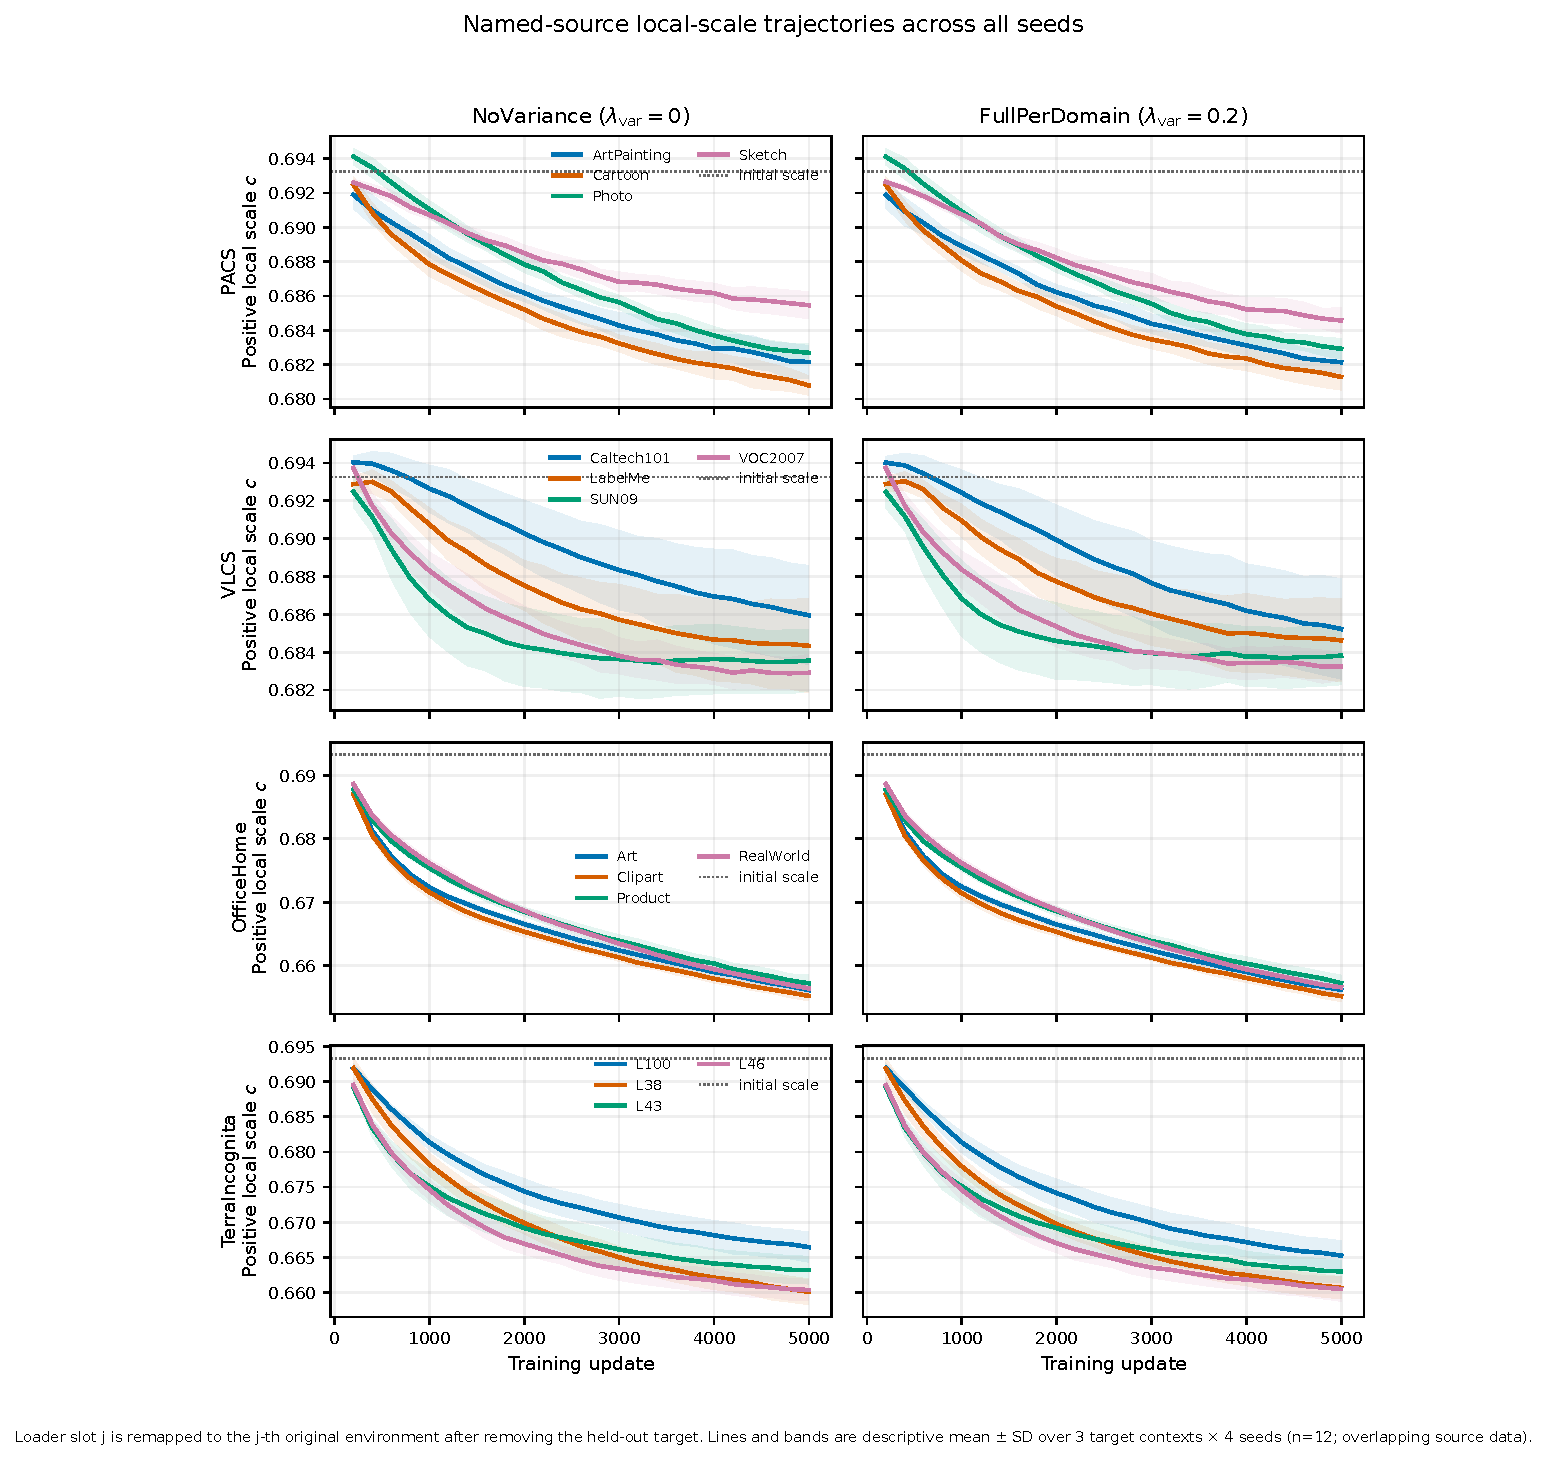
\includegraphics[width=\textwidth]{revision_assets/figures/curvature_scale_trajectories_named_all_seeds.pdf}
\caption{Learned local-scale trajectories for \full{} and \novar{}, aggregated
over all four run seeds and labeled by the named source represented by each
loader slot. Bands are descriptive mean $\pm$ SD over 12 overlapping
target-context/run-seed observations per named source and checkpoint, not
independent confidence intervals. The plotted positive values are Euclidean
feature scales, not learned sectional curvatures.}
\label{fig:scale-trajectories}
\end{figure}
}{}

\begin{table}[H]
\centering
\caption{Final within-run range across the three learned local scales. Each
cell gives the mean range over 16 target/seed runs followed by the maximum
range. This all-seed summary replaces the earlier seed-0-only diagnostic.}
\label{tab:scale-spread}
\small
\begin{tabular}{lrr}
\toprule
Dataset & \novar{} mean / max & \full{} mean / max \\
\midrule
PACS & 0.003837 / 0.005934 & 0.002667 / 0.004499 \\
VLCS & 0.003169 / 0.006600 & 0.002475 / 0.004947 \\
OfficeHome & 0.001482 / 0.002970 & 0.001445 / 0.002477 \\
TerraIncognita & 0.006020 / 0.010730 & 0.004476 / 0.008534 \\
\bottomrule
\end{tabular}
\end{table}

\subsection{SharedLearnable and global-scale trajectories}
\label{sec:shared-trajectories}

Figure~\ref{fig:scale-trajectories} above shows only \full{} and \novar{},
since those are the two conditions with three named per-source local scales.
\shared{} has a single learned local scale by construction, so it cannot be
decomposed by named source; to compare it against \novar{} on the same axis,
we summarize \novar{}'s three per-run local scales by their per-run mean. This
mean is a descriptive summary constructed only for this comparison, not a new
inferential estimand.

\IfFileExists{revision_assets/figures/curvature_scale_trajectories_shared_vs_novariance.pdf}{%
\begin{figure}[H]
\centering
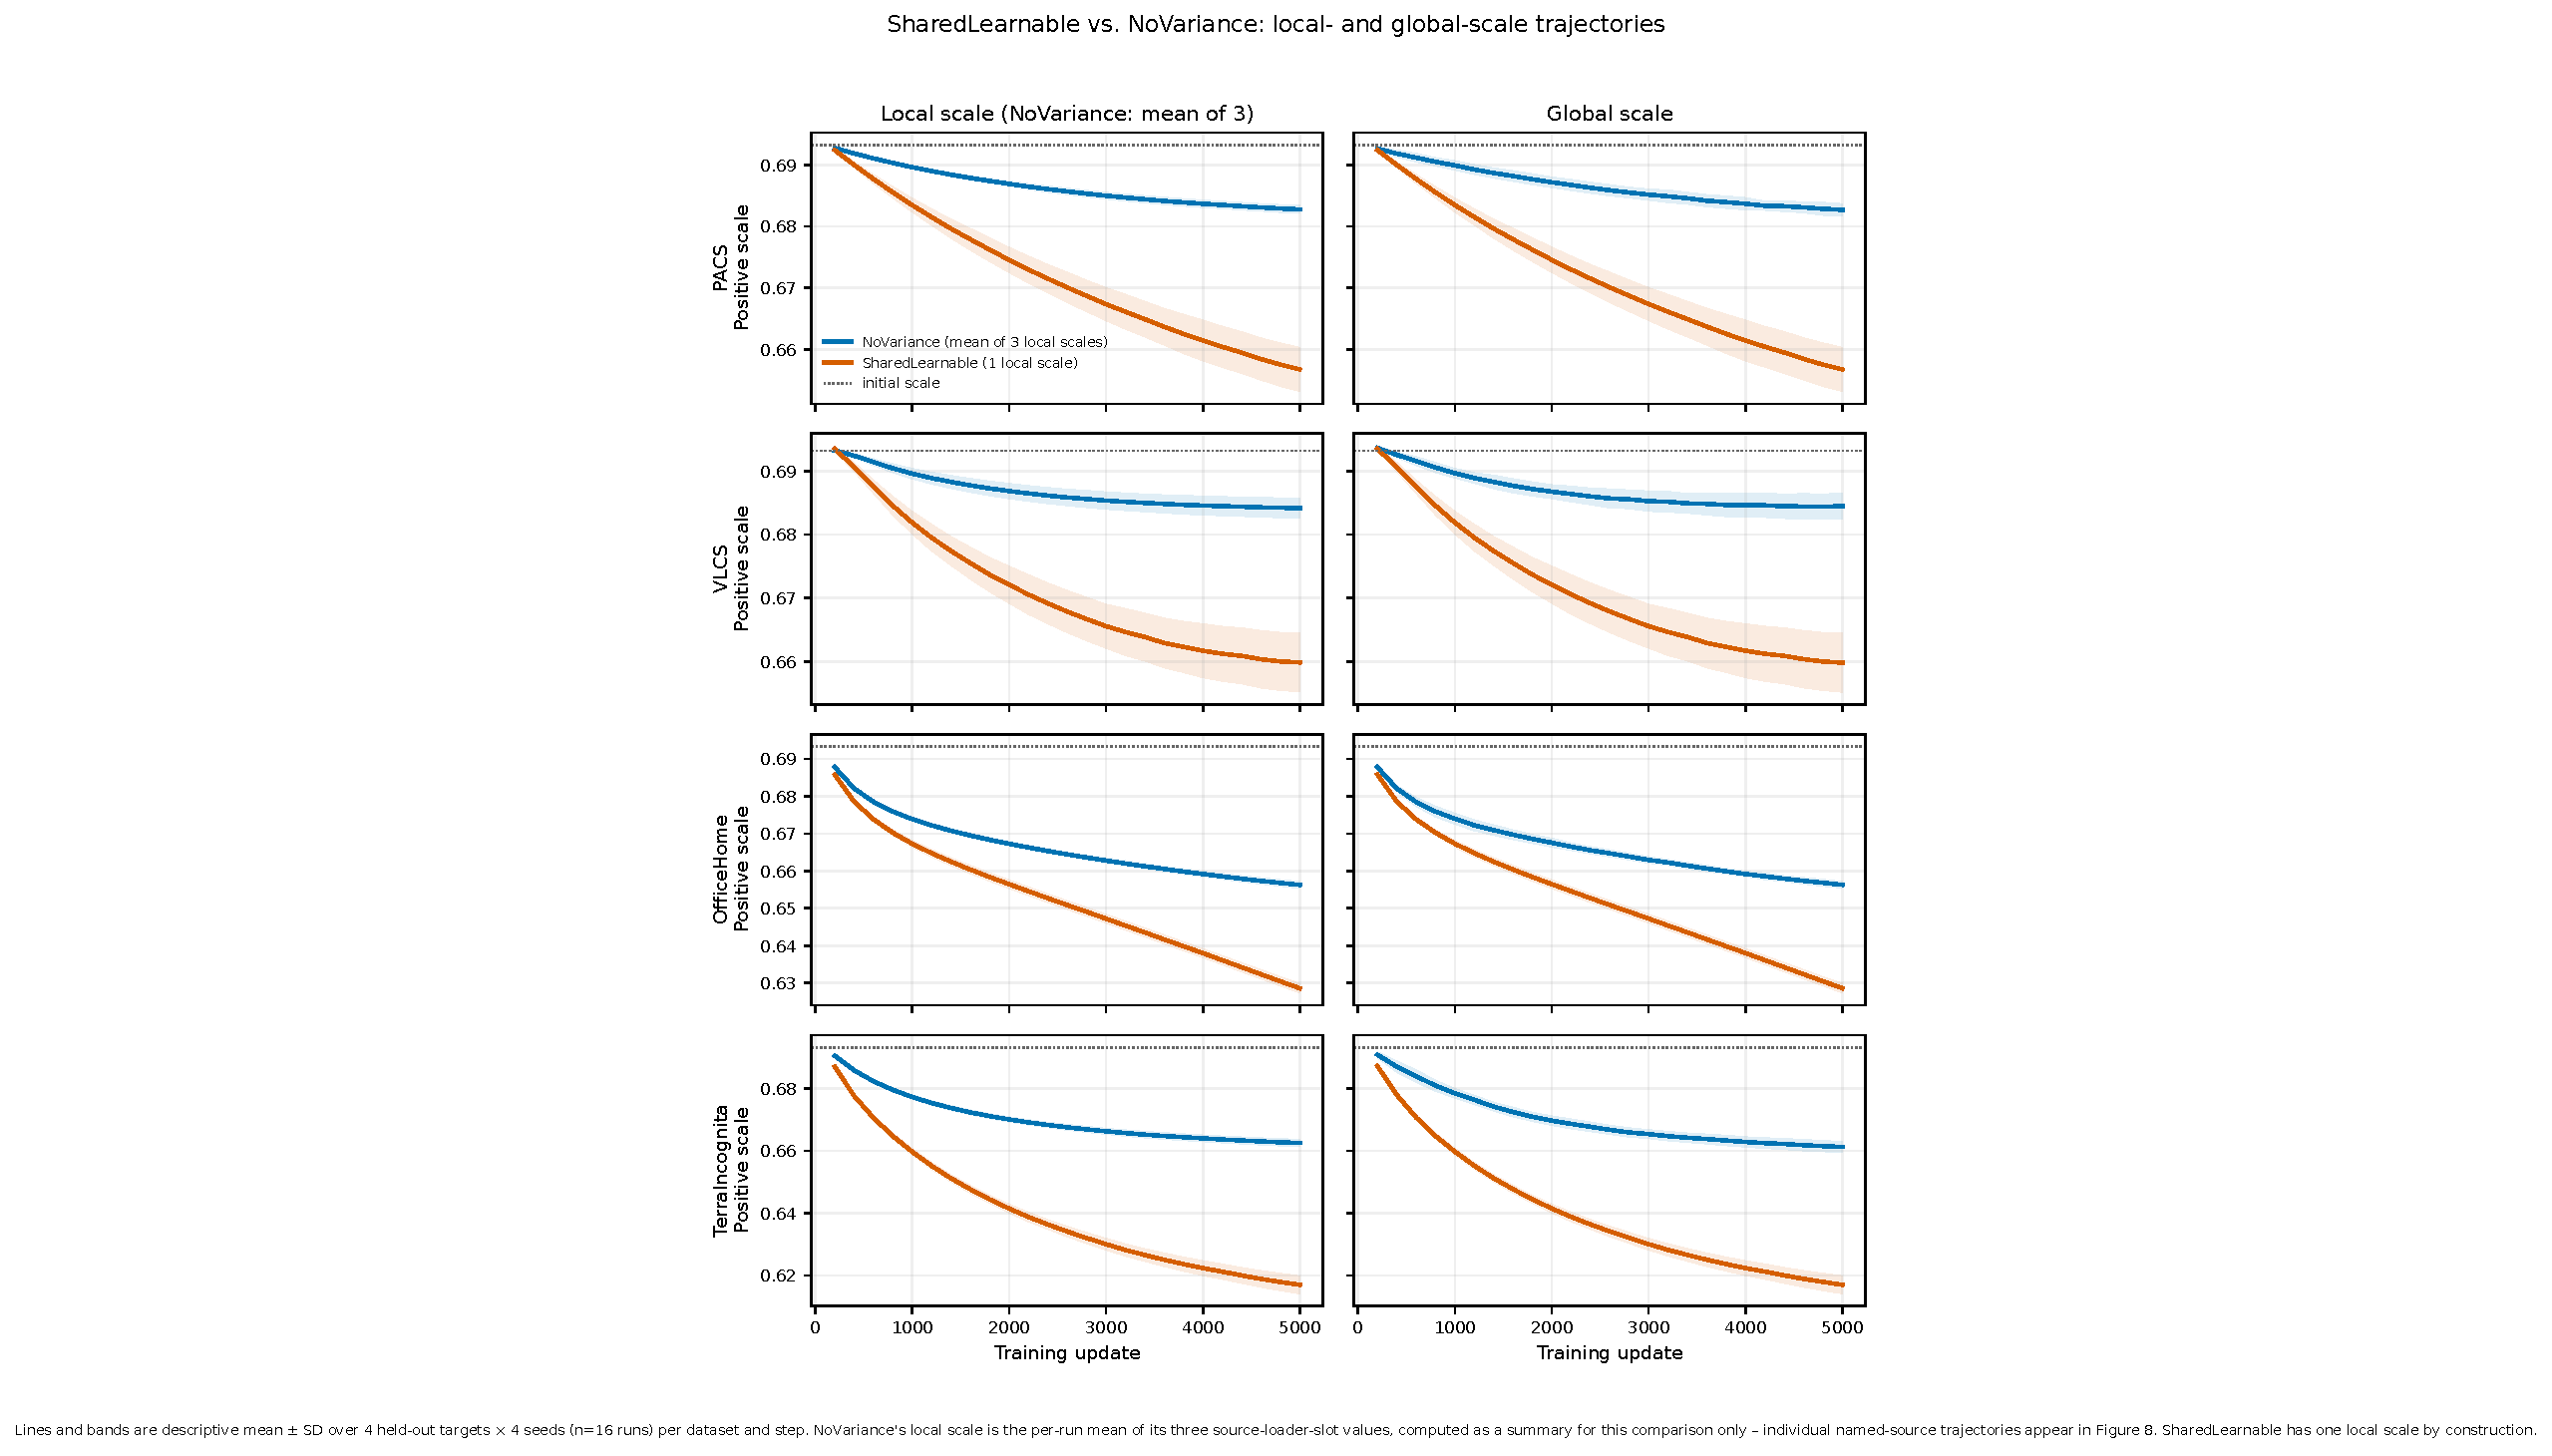
\includegraphics[width=\textwidth]{revision_assets/figures/curvature_scale_trajectories_shared_vs_novariance.pdf}
\caption{Local-scale (\novar{}'s per-run mean of three source-loader-slot
values vs.\ \shared{}'s single value) and global-scale trajectories,
aggregated over all four held-out targets and four run seeds (mean $\pm$ SD,
$n=16$ runs per dataset and checkpoint). Both conditions start every scale at
$0.693247$ (dotted line). Descriptively, \shared{}'s single local and global
scales move further from this initial value than \novar{}'s per-run mean
local scale does, on all four datasets; we do not treat this as evidence for
or against either parameterization; it is not one of the paper's two primary
contrasts, and Table~\ref{tab:primary-suite} already reports the
performance-based \novar{}$-$\shared{} equivalence result that is this
comparison's inferential counterpart.}
\label{fig:shared-vs-novar-trajectories}
\end{figure}
}{}

\subsection{BatchNorm and optimizer routes}

BatchNorm is not frozen. The \method{} update processes the three source
minibatches separately, then performs an additional no-gradient prediction
pass for a training diagnostic while remaining in train mode. Native ERM
concatenates source minibatches and performs one feature-extractor pass. The
routes therefore update running statistics differently. HyperDG also uses
separate Adam optimizers for network and scale parameters and clips both
gradient norms; native ERM retains its unmodified single optimizer without
that clipping. These differences are part of the treatment in
\full{}$-$\erm{}, which is why the paper calls it a package-utility comparison.

\section{Learning-Curve Diagnostics}
\label{sec:curves}

Target curves are generated after training for diagnosis and never enter the
selection function. Cross markers indicate checkpoints selected solely by mean
stochastic source-validation accuracy.

\begin{figure}[H]
\centering
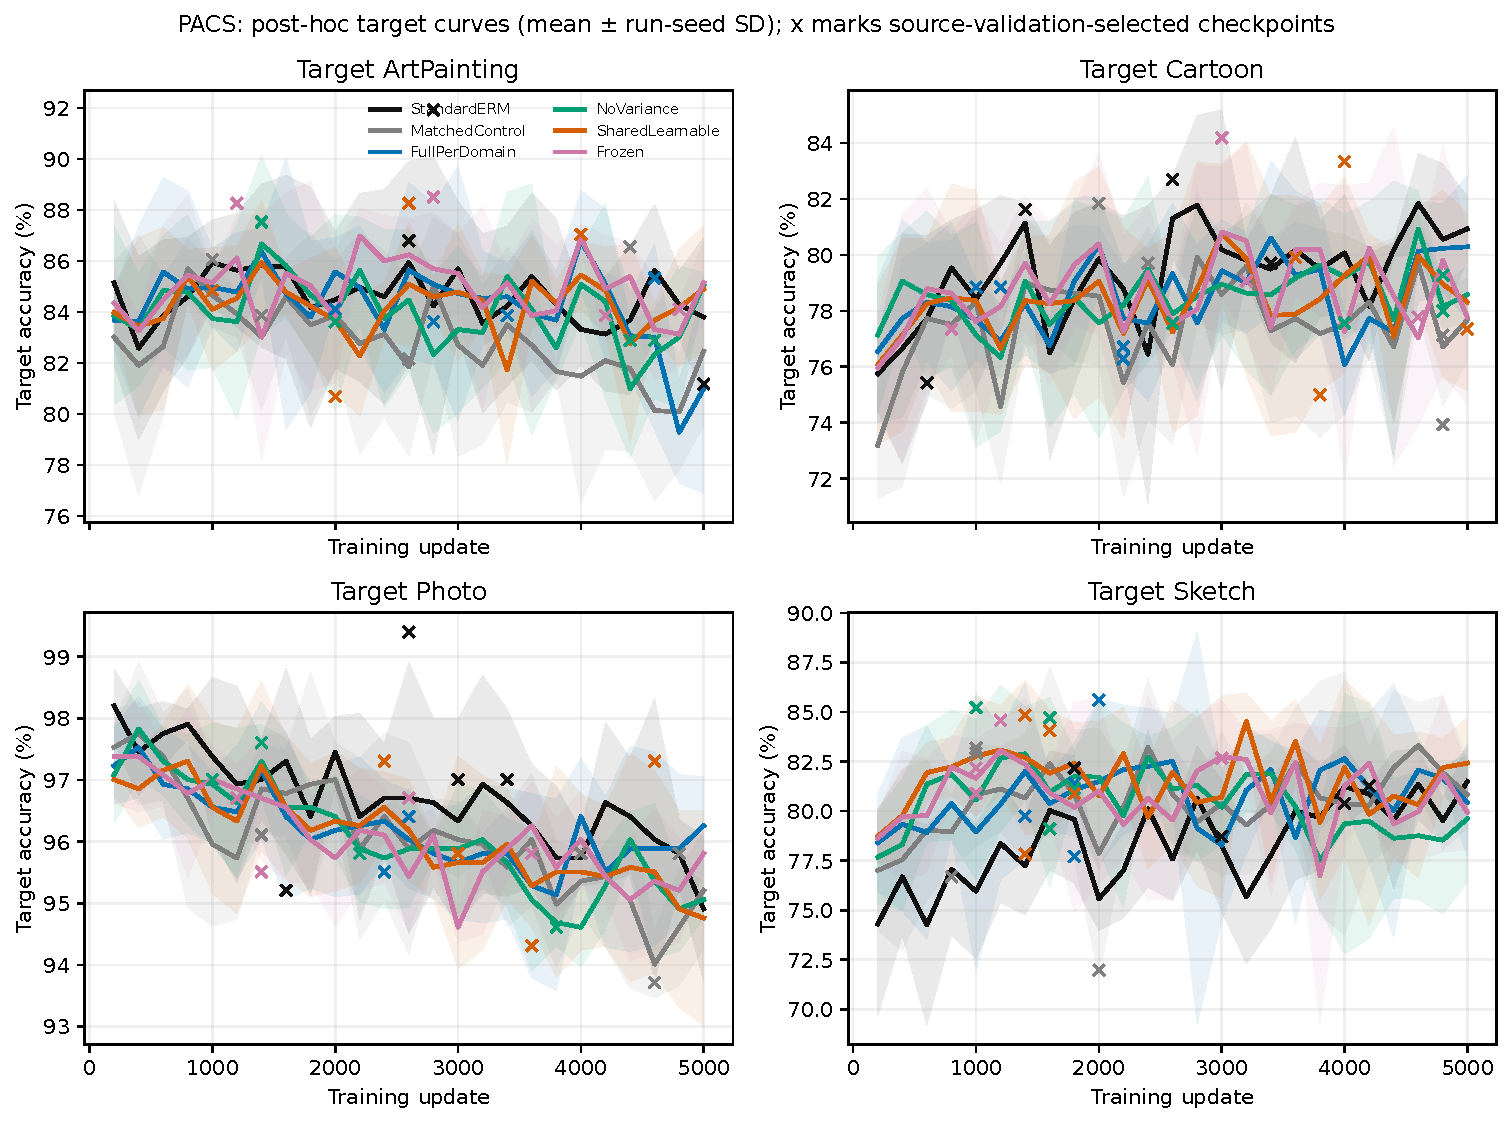
\includegraphics[width=0.49\textwidth]{revision_assets/figures/learning_curves_by_target_pacs.pdf}
\hfill
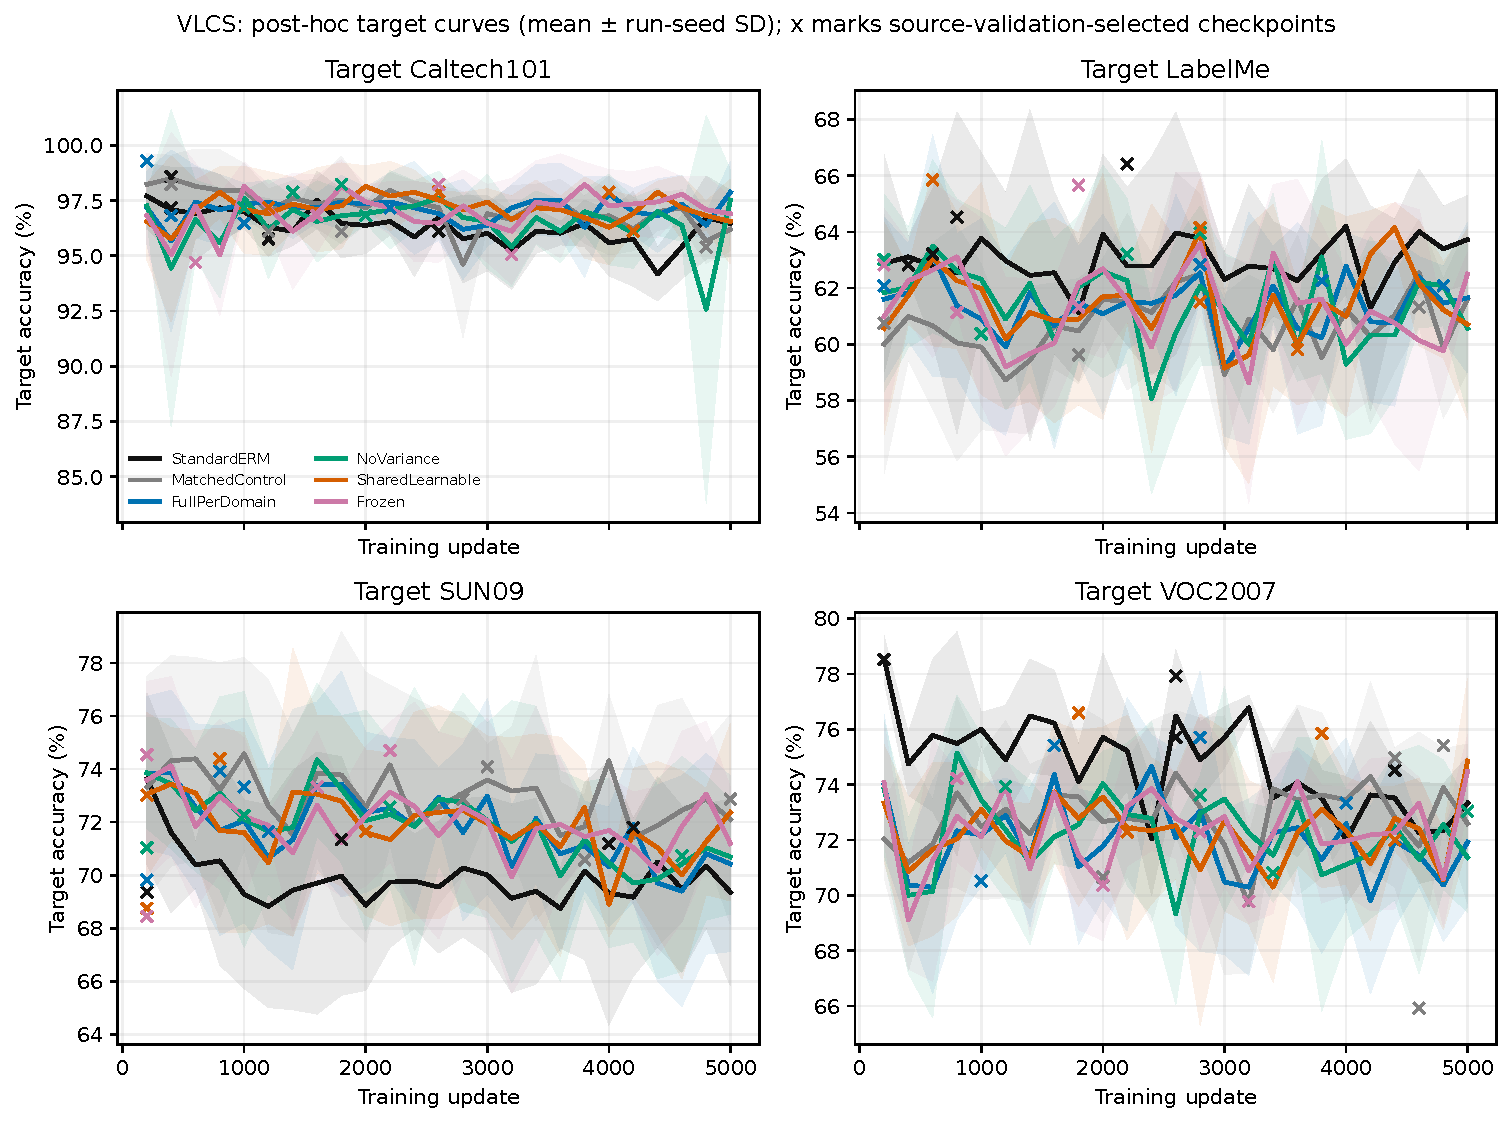
\includegraphics[width=0.49\textwidth]{revision_assets/figures/learning_curves_by_target_vlcs.pdf}
\caption{PACS and VLCS learning curves by named held-out target. Curves are
descriptive; checkpoint selection uses only source-validation accuracy.}
\label{fig:curves-pacs-vlcs}
\end{figure}

\begin{figure}[H]
\centering
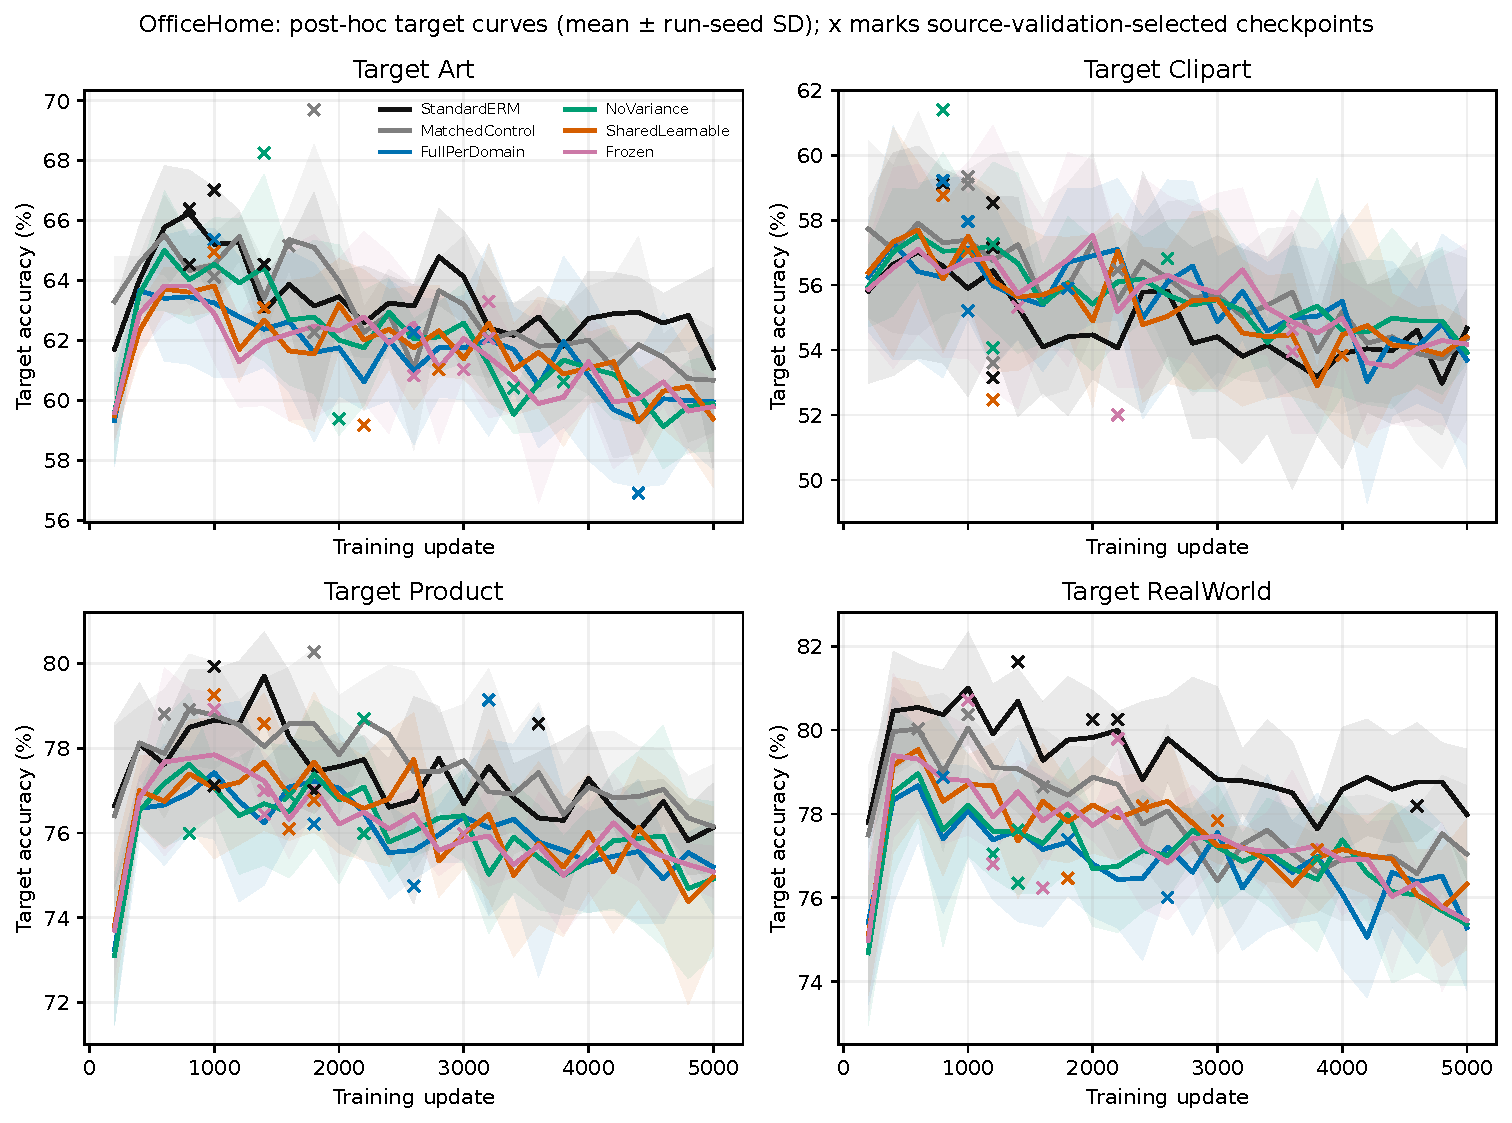
\includegraphics[width=0.49\textwidth]{revision_assets/figures/learning_curves_by_target_officehome.pdf}
\hfill
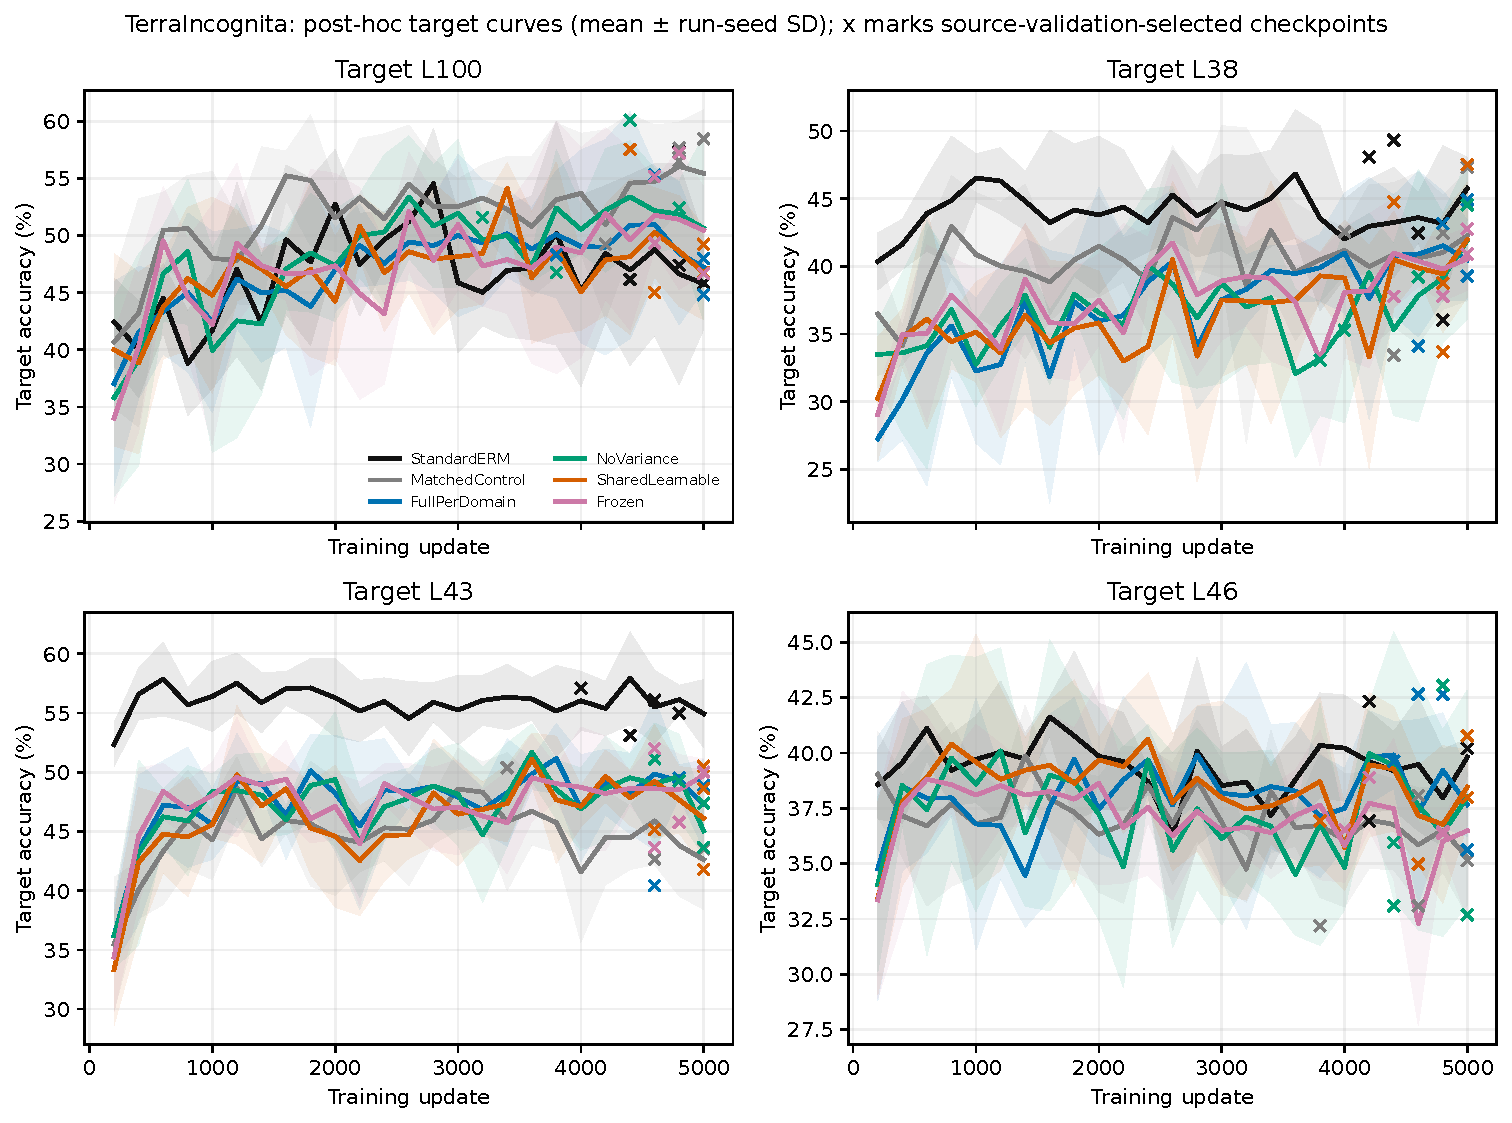
\includegraphics[width=0.49\textwidth]{revision_assets/figures/learning_curves_by_target_terraincognita.pdf}
\caption{OfficeHome and TerraIncognita learning curves by named held-out
target.}
\label{fig:curves-office-terra}
\end{figure}

\begin{figure}[H]
\centering
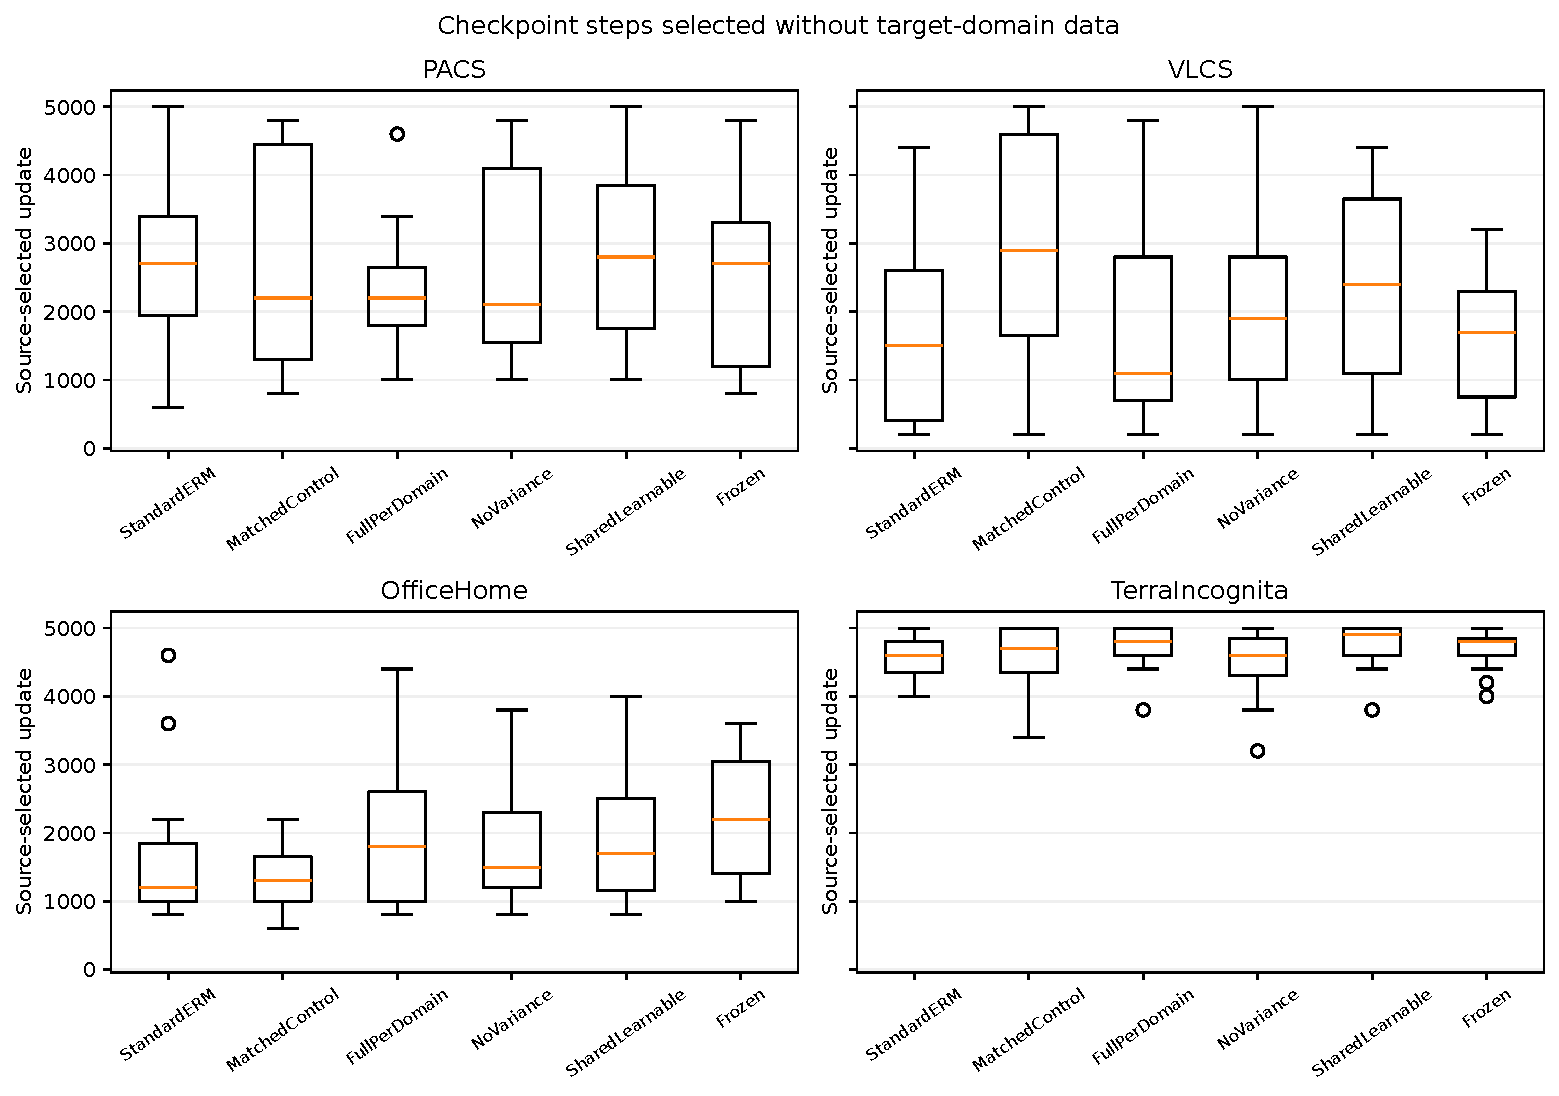
\includegraphics[width=0.86\textwidth]{revision_assets/figures/source_selected_steps.pdf}
\caption{Distribution of source-selected checkpoint steps by condition and
dataset.}
\label{fig:selected-steps}
\end{figure}

\section{Why the Existing Geometry Diagnostics Are Excluded}
\label{sec:excluded}

\begin{table}[H]
\centering
\caption{Disposition of geometry-related analyses outside the 384-run
controlled matrix.}
\label{tab:excluded}
\small
\begin{tabular}{p{0.26\linewidth}p{0.24\linewidth}p{0.42\linewidth}}
\toprule
Analysis & What it computes & Why it supports no main claim \\
\midrule
Post-hoc Poincar\'e projection & Maps already trained Euclidean features for a
two-dimensional visualization & Does not train a hyperbolic encoder or
classifier; projection appearance cannot validate learned curvature. \\
Legacy MERU adaptation & Partial attempt to add a Lorentz-style comparison &
Run grid is incomplete and not protocol-matched; it cannot answer the
reviewer's genuine-hyperbolic request. \\
Old seed-0 shared runs & One shared scalar in a mixed software environment &
Incomplete and environment-mismatched; replaced by all 64 fresh
\shared{} runs. \\
Frozen scales & Fixed scalars with other auxiliary terms active & Tests
learnability, not one learned shared scale; not used for domain specificity. \\
\bottomrule
\end{tabular}
\end{table}

A valid genuine-hyperbolic extension would implement a manifold-valued
Poincar\'e or Lorentz representation and appropriate classifier under the same
splits, seeds, backbone, budget, and target-excluding selector. It would need
fixed- and learned-curvature controls and the same target-clustered analysis.
No result in the current study meets that definition, so the paper makes no
claim about such methods.

\end{document}
